\documentclass[10pt]{article} % Sets the document class to 'article' with a font size of 12pt

\newcommand{\DocumentTitle}{Le second degré}
\newcommand{\DocumentTheme}{Algebre}
\newcommand{\DocumentType}{Cours}

\input{../../model/settings_cours.tex}

\begin{document}

\maketitle % Generates the title

\section{Les fonctions polynômes du second degré}

\subsection{Forme développée}

\definitions{}{
	On appelle fonction polynôme (ou trinôme) du second degré toute fonction $f$ définie sur $\R$ par
	$f(x)=ax^2+bx+c$ où $a$, $b$ et $c$ sont trois réel avec $a\not=0$. \\
	Les réels $a$, $b$ et $c$ sont appelés coefficients de la fonction.
}

\remarque{L'expression $ax^2+bx+c$ est dit forme développée de $f(x)$.}

\subsection{Forme canonique}

\theoreme{}{
	Toute fonction trinôme du second degré définie par $f(x)=ax^2+bx+c$ peut s'écrire sous une forme appelée
	canonique $f(x)=a(x-\alpha)^2+\beta$, avec $\alpha=-\dfrac{b}{2a}$ et $\beta=f(\alpha)$.
}

\subsection{Sens de variation}

\propriete{}{
	Soit $f$ une fonction définie sur $\mathbb{R}$ par $f(x)=a(x-\alpha)^2+\beta$.
	\begin{enumerate}[(i)]
		\item Cas où $a>0$ : la fonction $f$ est strictement décroissante sur $]-\infty;\alpha]$ puis strictement croissante sur $[\alpha;+\infty[$. La fonction $f$ admet un minimum égal à $\beta$ atteint en $x=\alpha$.
		\item Cas où $a<0$ : la fonction $f$ est strictement croissante sur $]-\infty;\alpha]$ puis strictement décroissante sur $[\alpha;+\infty[$. La fonction $f$ admet un maximum égal à $\beta$ atteint en $x=\alpha$.
	\end{enumerate}
}

\textbf{On retient :}
\vspace{0.5em}

\begin{minipage}{0.5\textwidth}
	\begin{tikzpicture}[baseline, scale=1, transform shape]
		% Configuration des styles de ligne et de texte
		\tkzTabInit[
			lgt = 1.5, 	% Largeur de la première colonne
			espcl = 2,	% Largeur de la deuxième colonne
		]{$x$/1, $f(x)$/1.5}{$-\infty$, $\alpha$, $+\infty$}
		% Contenu du tableau de variations
		\tkzTabVar{+/, -/$\beta$, +/}
	\end{tikzpicture}
	\vspace{0.5em} % Ajoute de l'espace avant le tikzpicture
	\par car $a > 0$ % Text on a new line 
\end{minipage}% <- This '%' sign is crucial to avoid unintended space
\begin{minipage}{0.5\textwidth}
	\begin{tikzpicture}[baseline, scale=1, transform shape]
		% Configuration des styles de ligne et de texte
		\tkzTabInit[
			lgt=1.5, % largeur entre les lignes
			espcl=2, % espacement des colonnes
		]{$x$/1, $f(x)$/1.5}{$-\infty$, $\alpha$, $+\infty$}
		% Contenu du tableau de variations
		\tkzTabVar{-/, +/$\beta$, -/}
	\end{tikzpicture}
	\vspace{0.5em} % Ajoute de l'espace avant le tikzpicture
	\par car $a < 0$ % Text on a new line 
\end{minipage}

\subsection{Représentation graphique}

\propriete{(conséquence)}{
	Soit $f$ une  fonction définie par $f(x)=a(x-\alpha)^2+\beta$. \\
	Dans un repère orthogonal d'origine $O$, la représentation graphique de la fonction $f$ est une parabole de sommet
	$S(\alpha;\beta)$ qui admet pour axe de symétrie la droite d'équation $x=\alpha$.
}

\newpage

\textbf{On retient :}
\vspace{0.5em}

\begin{minipage}{0.5\textwidth}
	\centering

	\begin{tikzpicture}
		\begin{axis}[
				axis lines=middle,
				xlabel={$x$}, ylabel={$y$},
				xmin=0, xmax=4,
				ymin=0, ymax=4,
				xtick={2},
				xticklabels={$\color{green}\alpha$},
				ytick={1},
				yticklabels={$\color{blue}\beta$},
				samples = 100
			]

			\addplot[green, densely dashed, thin] coordinates {(2,0) (2,5)}; % Courbe de x=2
			\addplot[blue, densely dashed, thin] {1}; % Courbe de y=1

			\addplot[red, thick] {(x - 2)^2 + 1}; % Courbe de f(x)
			\node[red] at (axis cs:3.25,3.75) {$f(x)$}; % Nom de f(x)

			\addplot[mark=*, black, mark size = 1.5, thick] coordinates {(2,1)};
			\node[black] at (axis cs:2.5,0.75) {$S(\green{\alpha};\blue{\beta})$}; % Nom de S(alpha;beta)
		\end{axis}
	\end{tikzpicture}

	\vspace{0.5em} % Ajoute de l'espace avant le tikzpicture
	\par car $a > 0$ % Text on a new line 
\end{minipage}% <- This '%' sign is crucial to avoid unintended space
\begin{minipage}{0.5\textwidth}
	\centering
	\begin{tikzpicture}
		\begin{axis}[
				axis lines=middle,
				xlabel={$x$}, ylabel={$y$},
				xmin=0, xmax=4,
				ymin=0, ymax=4,
				xtick={2},
				xticklabels={$\color{green}\alpha$},
				ytick={1},
				yticklabels={$\color{blue}\beta$},
				samples = 100
			]

			\addplot[green, densely dashed, thin] coordinates {(2,0) (2,5)}; % Courbe de x=2
			\addplot[blue, densely dashed, thin] {3}; % Courbe de y=1

			\addplot[red, thick] {-(x - 2)^2 + 3}; % Courbe de f(x)
			\node[red] at (axis cs:3.25,0.5) {$f(x)$}; % Nom de f(x)

			\addplot[mark=*, black, mark size = 1.5, thick] coordinates {(2,3)};
			\node[black] at (axis cs:2.5,3.25) {$S(\green{\alpha};\blue{\beta})$}; % Nom de S(alpha;beta)
		\end{axis}
	\end{tikzpicture}

	\vspace{0.5em} % Ajoute de l'espace avant le tikzpicture
	\par car $a < 0$ % Text on a new line 
\end{minipage}


\section{Factorisation d'une fonction du second degré et résolution d'équation du second degré}

\subsection{Factorisation}

\definition{}{
	On appelle discriminant de la fonction trinôme $f(x)=ax^2 + bx + c$ ou de l'équation $ax^2+bx+c=0$ le réel $\Delta$ défini
	par $\Delta=b^2-4ac$.
}

\theoreme{de factorisation d'un trinôme du second degré}{
	Soit $f$ définie sur $\R$ par $f(x)=ax^2+bx+c$.
	\begin{enumerate}[(i)]
		\item Si $\Delta<0$, alors $f(x)=ax^2+bx+c$ n'est pas factorisable.
		\item Si $\Delta=0$, alors $f(x)=a(x-\alpha)^2$ où $\alpha=-\dfrac{b}{2a}$.
		\item Si $\Delta>0$, alors $f(x)=a(x-x_1)(x-x_2)$ où  $x_1=\dfrac{-b-\sqrt{\Delta}}{2a}$ et $x_2=\dfrac{-b+\sqrt{\Delta}}{2a}$.
	\end{enumerate}
}

\subsection{Résolution des équation du second degré}

\theoreme{}{
	Soit l'équation $ax^2+bx+c=0$ avec $a\not=0$.
	\begin{enumerate}[(i)]
		\item Si $\Delta<0$, l'équation $ax^2+bx+c=0$ n'admet aucune solution.
		\item Si $\Delta=0$, l'équation $ax^2+bx+c=0$ admet une unique solution $\alpha=\dfrac{-b}{2a}$.
		\item Si $\Delta>0$, l'équation $ax^2+bx+c=0$ admet deux solutions distinctes : $x_1=\dfrac{-b-\sqrt{\Delta}}{2a}$ et $x_2=\dfrac{-b+\sqrt{\Delta}}{2a}$.
	\end{enumerate}
}

\subsection{Somme et produit des racines}

\propriete{}{
	Soit $x_1$ et $x_2$ les racines d'une fonction polynôme du second degré $f(x)=ax^2+bx+c$, avec $a\not=0$. \\
	On a alors $x_1+x_2=-\dfrac{b}{a}$ et $x_1\times x_2=\dfrac{c}{a}$
}

\section{Signe d'une fonction du second degré et inéquations}

\propriete{}{
	Soit $f$ définie sur $\mathbb{R}$ par $f(x)=ax^2+bx+c$.
	\begin{enumerate}[(i)]
		\item Si $\Delta<0$, alors pour tout réel $x$, $f(x)$ est du signe de $a$.
		\item Si $\Delta=0$, alors pour tout réel $x$, $f(x)$ est du signe de $a$ sauf en $\alpha$ où $f(x)=0$.
		\item Si $\Delta>0$, alors pour tout réel $x$, $f(x)$ s'annule en $x_1$ et $x_2$ et est du signe de $a$ pour
		      tout $x\in]-\infty;x_1[\cup]x_2;+\infty[$ avec $x_1<x_2$ et du signe opposé à celui de $a$ pour tout $x\in]x_1;x_2[$.
	\end{enumerate}
}

\remarque{On peut retenir que $f(x)$ est du signe de $a$ sauf entre les racines lorsqu'elles existent.}



\end{document}
